\section{The Domino compiler}
\label{s:compiler}

%TODO: Decide if we can add the figure before each point to make it more stylized.
% like (Figure XXX Branch removal).
The \pktlanguage compiler compiles from \pktlanguage programs to \absmachine
targets. The compiler provides an {\em all-or-nothing model}: if compilation
succeeds, the compiler guarantees that the program will run at line rate on the
target. If the program can't be run at line rate, the compiler rejects the
program outright; there is no smooth tradeoff between a program's performance
and its complexity.  This all-or-nothing compilation model is unusual relative
to other substrates such as a CPU, GPU, or DSP. But, it reflects how routers
are used today. Routers are rated for a particular line rate, regardless of the
enabled feature set. The all-or-nothing model trades off diminished
programmability for guaranteed line-rate performance, in contrast to software
routers that provide greater flexibility but unpredictable run-time
performance~\cite{dobrescu2012, wenfei15}.

The \pktlanguage compiler has three passes (Figure~\ref{fig:passes}).  First,
\textit{normalization} simplifies the packet transaction into a restrictive
three-address code form while retaining the sequential nature of packet
transactions, i.e., processing one packet at a time. Second, \textit{pipelining} transforms the normalized code into
code for a \textit{pipelined virtual switch machine (PVSM)}. PVSM is an
intermediate representation that models a switch pipeline with no computational
or resource limits. Third, \textit{code generation} transforms this
intermediate representation into configuration for a \absmachine machine, given
as inputs the machine's computational and resource constraints, and rejects the
program if it can't run at line rate on that \absmachine machine.  The
\pktlanguage compiler uses many existing compiler techniques, but adapts and
simplifies them in important ways to suit the domain of line-rate switches
(\S\ref{ss:related_compiler}). Throughout this section, we use flowlet
switching as a running example to demonstrate compiler passes.

\begin{figure}[!t]
  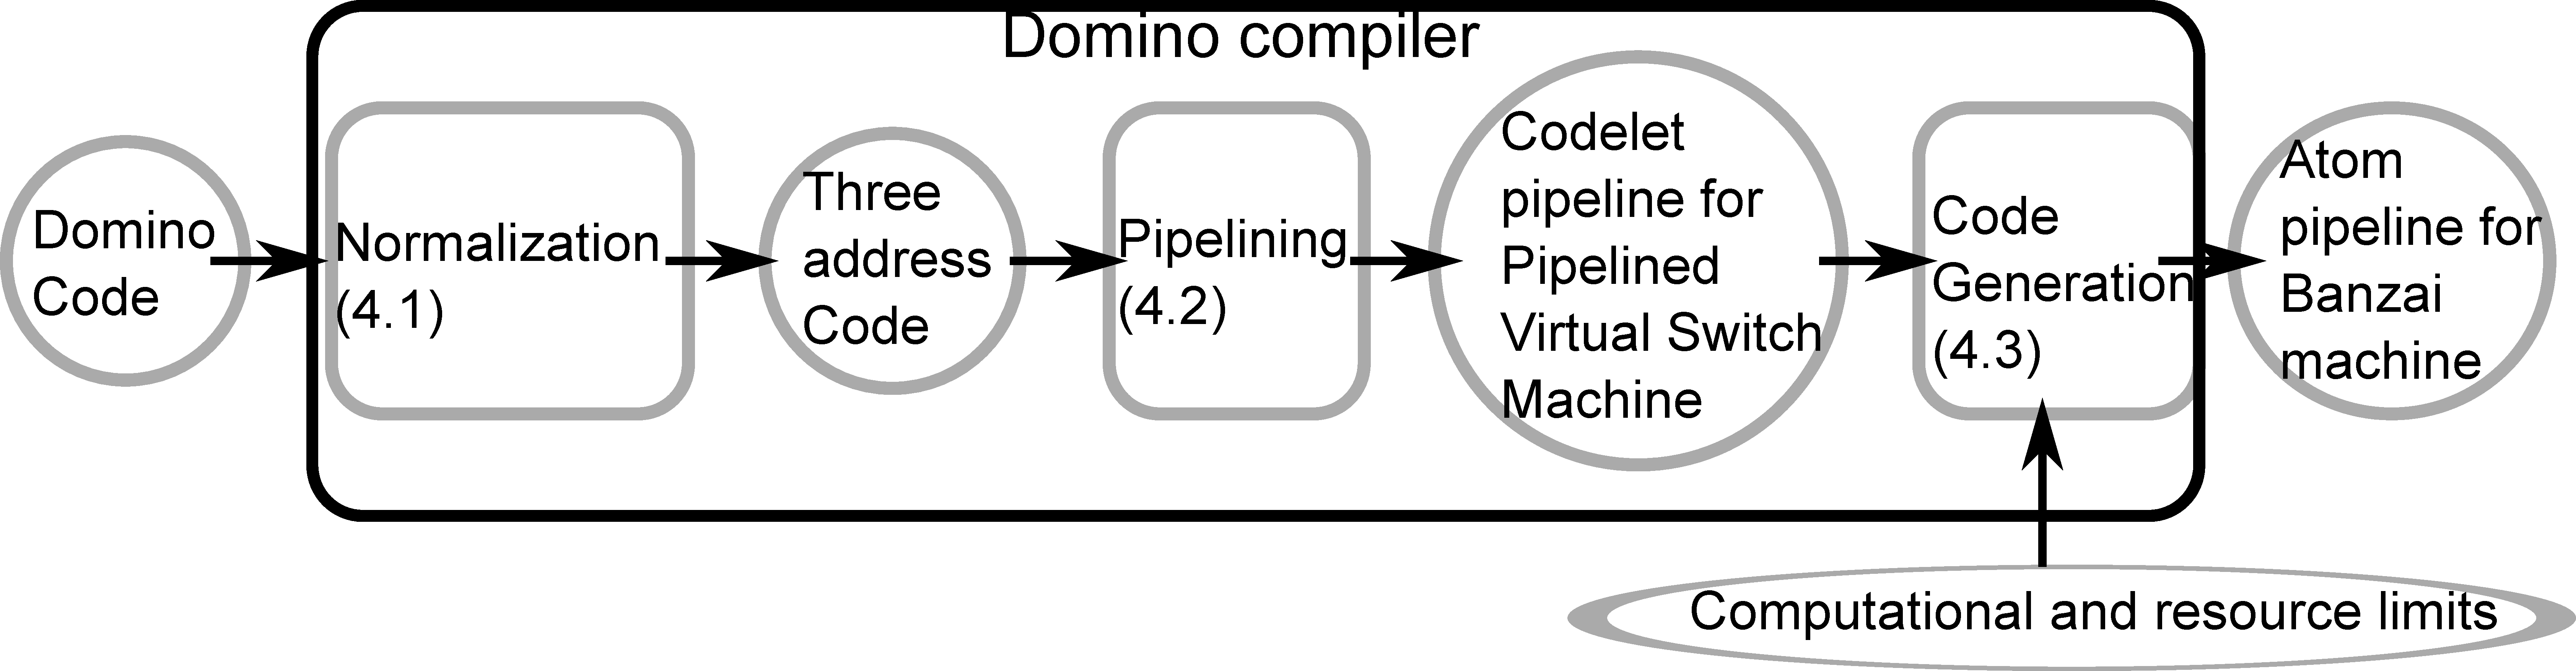
\includegraphics[width=\columnwidth]{compiler-fig.pdf}
  \caption{Passes in the \pktlanguage compiler}
  \label{fig:passes}
\end{figure}

\subsection{Normalization}
\label{ss:normalization}

\textbf{Branch removal: }A packet transaction's body can contain (potentially
nested) branches (e.g., Lines~\ref{line:ifStart} to \ref{line:ifEnd} in
Figure~\ref{fig:flowlet_code}).  Branches alter control flow and complicate
dependency analysis, i.e.,  whether a statement should precede another.  We
transform branches into the conditional operator, starting from the innermost
\texttt{if} and recursing outwards (Figure~\ref{fig:if_convert}).  This turns
the transaction body into straight-line code with no branches.  Straight-line
code simplifies the rest of the compiler, by simplifying dependency analysis
and conversion to static single-assignment form.

\textbf{Rewriting state variable operations: }We now identify state variables
in a packet transaction, such as \texttt{last\_time} and \texttt{saved\_hop} in
Figure~\ref{fig:flowlet_code}.  For each state variable, we create a
\textit{read flank} to read the state variable into a temporary packet field.
For an array, we also move the index expression into the read flank using the
fact that only one array index is accessed by each packet.  Within the packet
transaction, we replace the state variable with the packet temporary, and
create a \textit{write flank} to write the packet temporary back into the state
variable~(Figure~\ref{fig:stateful_flanks}). After this, the only operations
on state variables are reads and writes; all arithmetic happens on packet
fields. Restricting stateful operations simplifies handling of state during
pipelining.

\textbf{Converting to static single-assignment form: }We next convert the code to
static single-assignment form (SSA)~\cite{ssa}, where every packet field is
assigned exactly once. To do so, we replace every assignment to a packet field
with a new packet field and propagate this until the next assignment to the
same field~(Figure~\ref{fig:ssa}) .  Because every field is assigned exactly
once, SSA removes Write-After-Read and Write-After-Write dependencies.  Only
Read-After-Write dependencies remain, simplifying dependency analysis.

\textbf{Flattening to three-address code: } Three-address code~\cite{tac} is a
representation where all instructions are either reads/writes into state
variables or operations on packet fields of the form \texttt{pkt.f1 = pkt.f2 op
pkt.f3;} where \texttt{op} can be an arithmetic, logical, relational, or conditional
\footnote{Conditional operations alone have 4 arguments.} operator.  We also allow either one of {\tt pkt.f2} or {\tt pkt.f3}
to be an intrinsic function call.  To convert to three-address code, we flatten
expressions that are not in three-address code using
temporaries~(Figure~\ref{fig:three_address}).

%%Flattening may result in
%%temporaries that compute the same expression; we remove these using common
%%subexpression elimination~\cite{cse}.
%\footnote{Ternary/Conditional operators take in 4 addresses instead
%of 3.}
%%%\MA{Do we need a figure for every step? They're taking a lot of space,
%%%  and I feel weaving through them disrupts the flow of the paper. One
%%%  option is to only show the final result of the normalization stage
%%%  (Figure 8) and move all the intermediate figures to an Appendix}

\subsection{Pipelining}
\label{ss:partitioning}
At this point, the normalized code is still sequential in that it operates on a
single packet at a time without using a pipeline to process packets
concurrently.  Pipelining turns sequential code into a pipeline of
\textit{codelets}, where each codelet is a sequential block of three-address
code statements. This codelet pipeline corresponds to an intermediate
representation (IR) we call the \textit{Pipelined Virtual Switch Machine
(PVSM)}. PVSM places no computational or resource constraints on the
pipeline---much like IRs such as LLVM place no restriction on the number of
virtual registers. Later, during code generation, we map these codelets to
atoms available in a \absmachine machine, while respecting its constraints.

We create PVSM's codelet pipeline using the steps below.
\begin{CompactEnumerate}
  \item Create a dependency graph of all statements in the normalized packet
    transaction. First, create a node for each statement. Second,
    add a pair of edges between any two nodes N1 and N2, where N1 is a read
    from a state variable and N2 is a write into the same variable, to capture
    the notion that state should be internal to a codelet/atom. Third, create
    an edge (N1, N2) for every pair of nodes N1, N2 where N2 reads a variable
    written by N1.  We only check read-after-write dependencies because we
    eliminate control dependencies\footnote{An instruction A is control
    dependent on a preceding instruction B if the outcome of B determines
    whether A should be executed or not.} through branch removal, and
    write-after-read and write-after-write dependencies don't exist after SSA.
    Figure~\ref{fig:partitioning_before} shows the resulting dependency graph.
  \item Generate strongly connected components (SCCs) of this dependency graph
    and condense them into a directed acyclic graph (DAG). This captures the notion that all
    operations on a state variable must be confined to one codelet/atom because
    state cannot be shared between atoms. Figure~\ref{fig:partitioning_after}
    shows the resulting DAG.
  \item Schedule the resulting DAG using critical path
    scheduling~\cite{crit_path_sched} by creating a new pipeline stage when one
    operation needs to follow another. This results in the codelet pipeline
    shown in Figure~\ref{fig:flowlet_pipeline}.\footnote{We refer to this both
    as a codelet and an atom pipeline because codelets map one-to-one atoms
  (\S\ref{ss:code_gen}).}
\end{CompactEnumerate}

The codelet pipeline implements the packet transaction on a switch pipeline
with no computational or resource constraints. We handle these constraints
next.

\subsection{Code generation}
\label{ss:code_gen}

To determine if the codelet pipeline can be compiled to a \absmachine machine,
we consider two constraints in any \absmachine machine: resource limits, i.e.,
the pipeline width and depth, and computational limits on atoms within a
pipeline stage, i.e., the atom templates provided by a \absmachine machine.

\textbf{Resource limits:} To handle resource limits, we scan each pipeline
stage in the codelet pipeline starting from the first to check for pipeline
width violations.  If we violate the pipeline width, we insert as many new
stages as required and spread codelets evenly across these stages.  We continue
until the number of codelets in all stages is under the pipeline width and
reject the program if we exceed the pipeline depth.

\textbf{Computational limits:} Next, we determine if codelets in the pipeline
map one-to-one to atoms provided by the \absmachine machine. In general,
codelets have multiple three-address code statements that need to execute
atomically. For instance, updating the state variable \texttt{saved\_hop} in
Figure~\ref{fig:flowlet_pipeline} requires a read followed by a conditional
write.  It is not apparent whether such codelets can be mapped to an available
atom. We develop a new technique to determine the implementability of a codelet,
given an atom template.

Each atom template has a set of configuration parameters, where the parameters
determine the atom's behavior.  For instance, Figure~\ref{fig:alu_diag} shows a
hardware circuit that can perform stateful addition or subtraction, depending
on the value of the constant and which output is selected from the multiplexer.
Its atom template is shown in Figure~\ref{fig:alu_in_sketch}, where {\tt
choice} and {\tt constant} represent configuration parameters.  Each codelet
can be viewed as a functional specification of the atom.  With that in mind,
the mapping problem is equivalent to searching for the value of the parameters
to configure the atom such that it implements the provided specification.

We use the SKETCH program synthesizer~\cite{sketch_asplos} for this purpose, as
the atom templates can be easily expressed using SKETCH, while SKETCH also
provides efficient search algorithms and has been used for similar purposes in
other domains~\cite{bitstreaming, lifejoin, qbs, chlorophyll}.  As an
illustration, assume we want to map the codelet {\tt x=x+1} to the atom
template shown in Figure~\ref{fig:alu_in_sketch}. SKETCH will search for
possible parameter values so that the resulting atom is functionally identical
to the codelet, for all possible input values of {\tt x}.  In this case, SKETCH
finds the solution with {\tt choice=0} and {\tt constant=1}.  In contrast, if
the codelet {\tt x=x*x} was supplied as the specification, SKETCH will return
an error as no parameters exist.

%TODO: George's suggestion motivating SKETCH.

%%To minimize search time, the range
%%of possible inputs and parameter values need to be specified in the template
%%(e.g., all 8 bit integers), and our experiments show that the search finishes
%%quickly, taking 10 secs at most.

%%\begin{figure}[!b]
%%  \begin{center}
%%  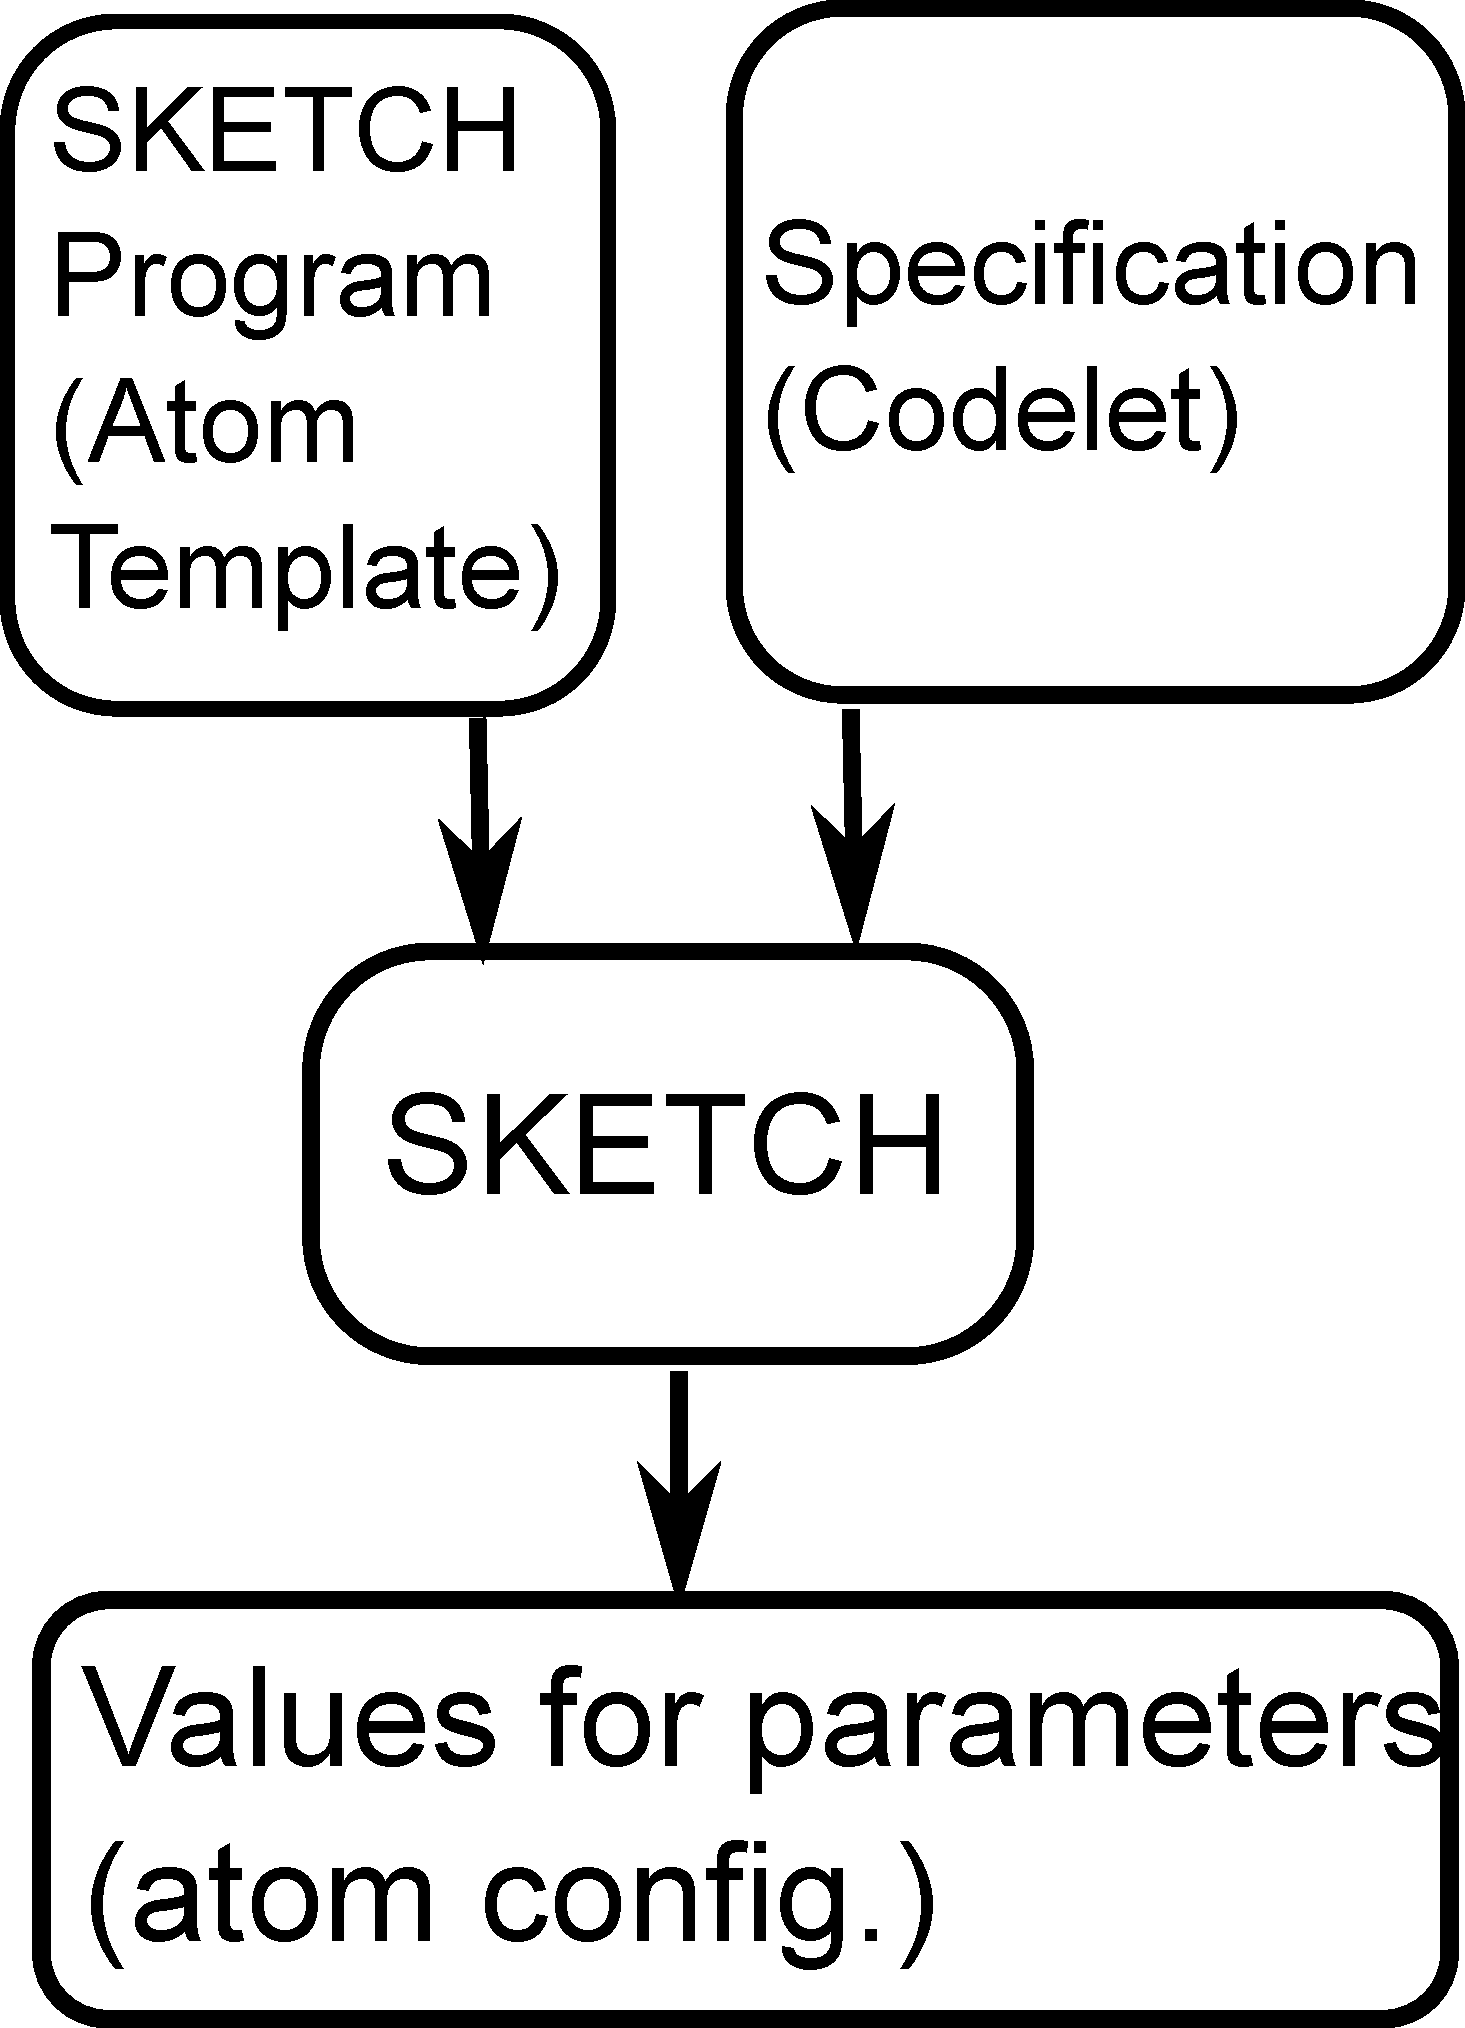
\includegraphics[width=0.4\columnwidth]{sketch.pdf}
%%  \caption{Overview of SKETCH and its application to atom configuration}
%%  \label{fig:sketch}
%%  \end{center}
%%\end{figure}

\begin{figure*}[!t]
  \hspace{-0.3in}
  \begin{minipage}{0.55\textwidth}
  \begin{small}
  \begin{lstlisting}[style=customc, numbers=none, frame=none]
  if (@\textcolor{blue}{pkt.arrival - last\_time[pkt.id] > THRESHOLD}@) {
    saved_hop[pkt.id] = pkt.new_hop;
  }
  \end{lstlisting}
  \end{small}
  \end{minipage}
%  
  \hspace{-0.5in}
  $\Longrightarrow$ 
  \hspace{-0.3in}
%  
  \begin{minipage}{0.6\textwidth}
  \begin{small}
  \begin{lstlisting}[style=customc, numbers=none, frame=none]
  @\textcolor{blue}{pkt.tmp = pkt.arrival - last\_time[pkt.id]  > THRESHOLD}@;
  saved_hop[pkt.id] = @\textcolor{blue}{pkt.tmp}@
                      ? pkt.new_hop
                      : saved_hop[pkt.id]; @\textcolor{magenta}{// Rewritten}@
  \end{lstlisting}
  \end{small}
  \end{minipage}
%\vspace{-.2in}
\caption{Branch removal}
\label{fig:if_convert}
\end{figure*}

\begin{figure*}[!t]
  \begin{minipage}{0.43\textwidth}
  \begin{small}
  \begin{lstlisting}[style=customc, numbers=none, frame=none]
pkt.id = hash2(pkt.sport,
               pkt.dport)
         % NUM_FLOWLETS;
...
@\textcolor{blue}{last\_time[pkt.id] = pkt.arrival;}@
...
  \end{lstlisting}
  \end{small}
  \end{minipage}
%  
  \hspace{-0.5in}
  $\Longrightarrow$ 
  \hspace{-0.2in}
%  
  \begin{minipage}{0.61\textwidth}
  \begin{small}
  \begin{lstlisting}[style=customc, numbers=none, frame=none]
pkt.id = hash2(pkt.sport,           @\textcolor{magenta}{// Read flank}@
               pkt.dport)
         % NUM_FLOWLETS;
pkt.last_time = last_time[pkt.id];  @\textcolor{magenta}{// Read flank}@
...
@\textcolor{blue}{pkt.last\_time = pkt.arrival;}@             @\textcolor{magenta}{// Rewritten}@
...
last_time[pkt.id] = pkt.last_time;  @\textcolor{magenta}{// Write flank}
  \end{lstlisting}
  \end{small}
  \end{minipage}
  \caption{Rewriting state variable operations}
\label{fig:stateful_flanks}
\end{figure*}

\begin{figure*}[!t]
  \begin{minipage}{\textwidth}
  \begin{minipage}{0.4\textwidth}
  \begin{small}
  \begin{lstlisting}[style=customc, numbers=none, frame=none]
@\textcolor{blue}{pkt.id}@ = hash2(pkt.sport,
              pkt.dport)
              % NUM_FLOWLETS;
@\textcolor{blue}{pkt.last\_time}@ = last_time[@\textcolor{blue}{pkt.id}@];
...
@\textcolor{blue}{pkt.last\_time}@ = pkt.arrival;
last_time[@\textcolor{blue}{pkt.id}@] = @\textcolor{blue}{pkt.last\_time}@;
  \end{lstlisting}
  \end{small}
  \end{minipage}
 % 
  %\hspace{-0.1in}
  $\Longrightarrow$
  \hspace{-0.2in}
%
  \begin{minipage}{0.6\textwidth}
  \begin{small}
  \begin{lstlisting}[style=customc, numbers=none, frame=none]
@\textcolor{blue}{pkt.id0}@ = hash2(pkt.sport,          @\textcolor{magenta}{// Rewritten}@ @\label{line:assign}@
               pkt.dport)
               % NUM_FLOWLETS;  
@\textcolor{blue}{pkt.last\_time0}@ = last_time[@\textcolor{blue}{pkt.id0}@];  @\textcolor{magenta}{// Rewritten}@
...
@\textcolor{blue}{pkt.last\_time1}@ = pkt.arrival;        @\textcolor{magenta}{// Rewritten}@
last_time[@\textcolor{blue}{pkt.id0}@] = @\textcolor{blue}{pkt.last\_time1}@;  @\textcolor{magenta}{// Rewritten}@
  \end{lstlisting}
  \end{small}
  \end{minipage}
  \caption[title]{Converting to static single-assignment form}
  \label{fig:ssa}
\end{minipage}
\end{figure*}


\begin{figure*}[!t]
\begin{minipage}{\textwidth}
\begin{lstlisting}[style=customc]
pkt.id            = hash2(pkt.sport, pkt.dport) % NUM_FLOWLETS; @\label{line:id}@
pkt.saved_hop     = saved_hop[pkt.id]; @\label{line:stateRead}@
pkt.last_time     = last_time[pkt.id];
pkt.new_hop       = hash3(pkt.sport, pkt.dport, pkt.arrival) % NUM_HOPS; @\label{line:newhop}@
pkt.tmp           = pkt.arrival - pkt.last_time;
pkt.tmp2          = pkt.tmp > THRESHOLD;
pkt.next_hop      = pkt.tmp2 ? pkt.new_hop : pkt.saved_hop;
saved_hop[pkt.id] = pkt.tmp2 ? pkt.new_hop : pkt.saved_hop; @\label{line:stateWrite}@
last_time[pkt.id] = pkt.arrival;
\end{lstlisting}
\caption[title2]{Flowlet switching in three-address
code. Lines~\ref{line:id} and \ref{line:newhop} are flipped relative
to Figure~\ref{fig:flowlet_code} because {\tt pkt.id} is an array index expression and is
moved into the read flank.}
\label{fig:three_address}
\end{minipage}
\vspace{-0.3cm}
\end{figure*}

\begin{figure*}[!t]
\begin{subfigure}{0.5\textwidth}
  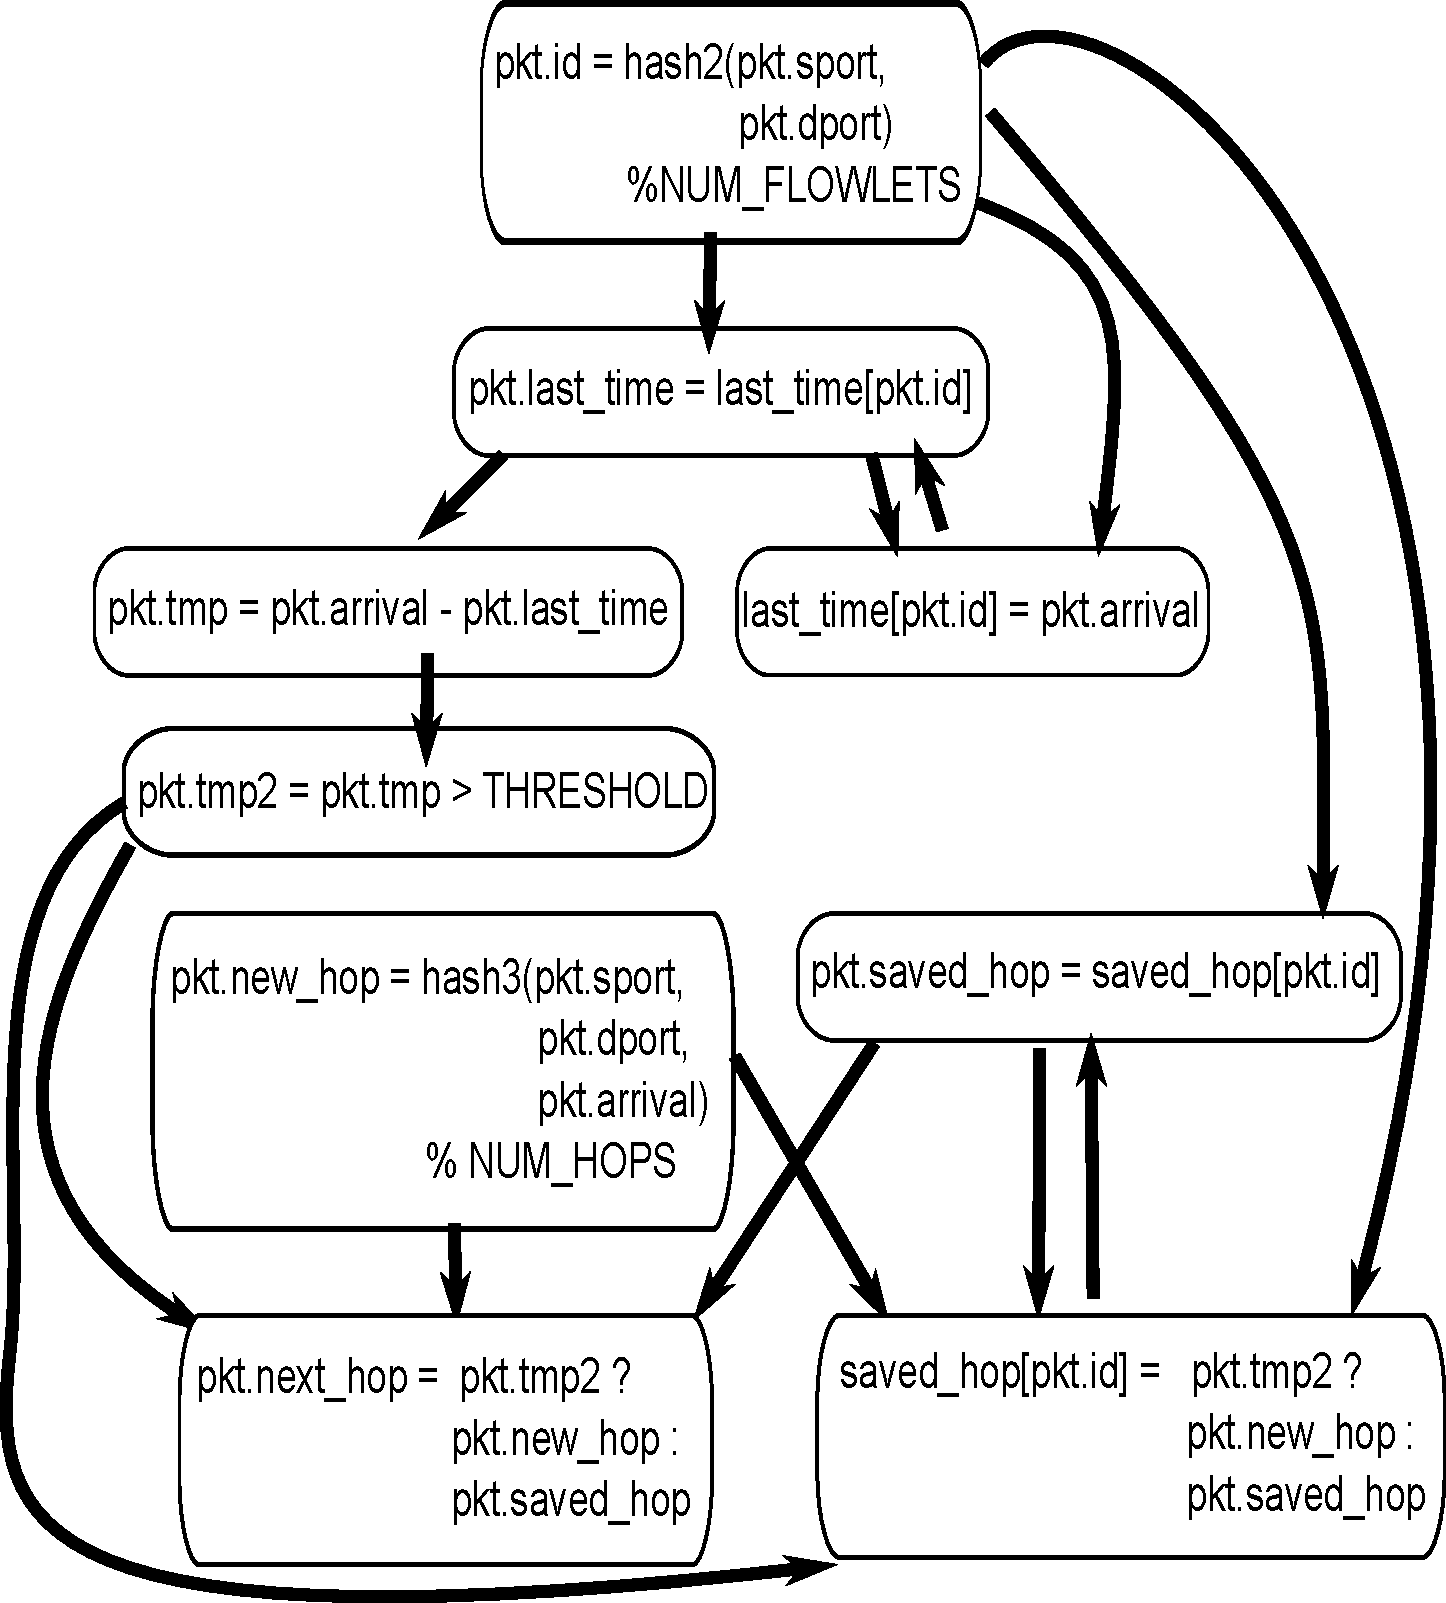
\includegraphics[width=0.8\columnwidth]{deps.pdf}
  \caption{Dependency graph. Edges are read-after-write dependencies.}
  \label{fig:partitioning_before}
\end{subfigure}
$\Longrightarrow$ 
\begin{subfigure}{0.5\textwidth}
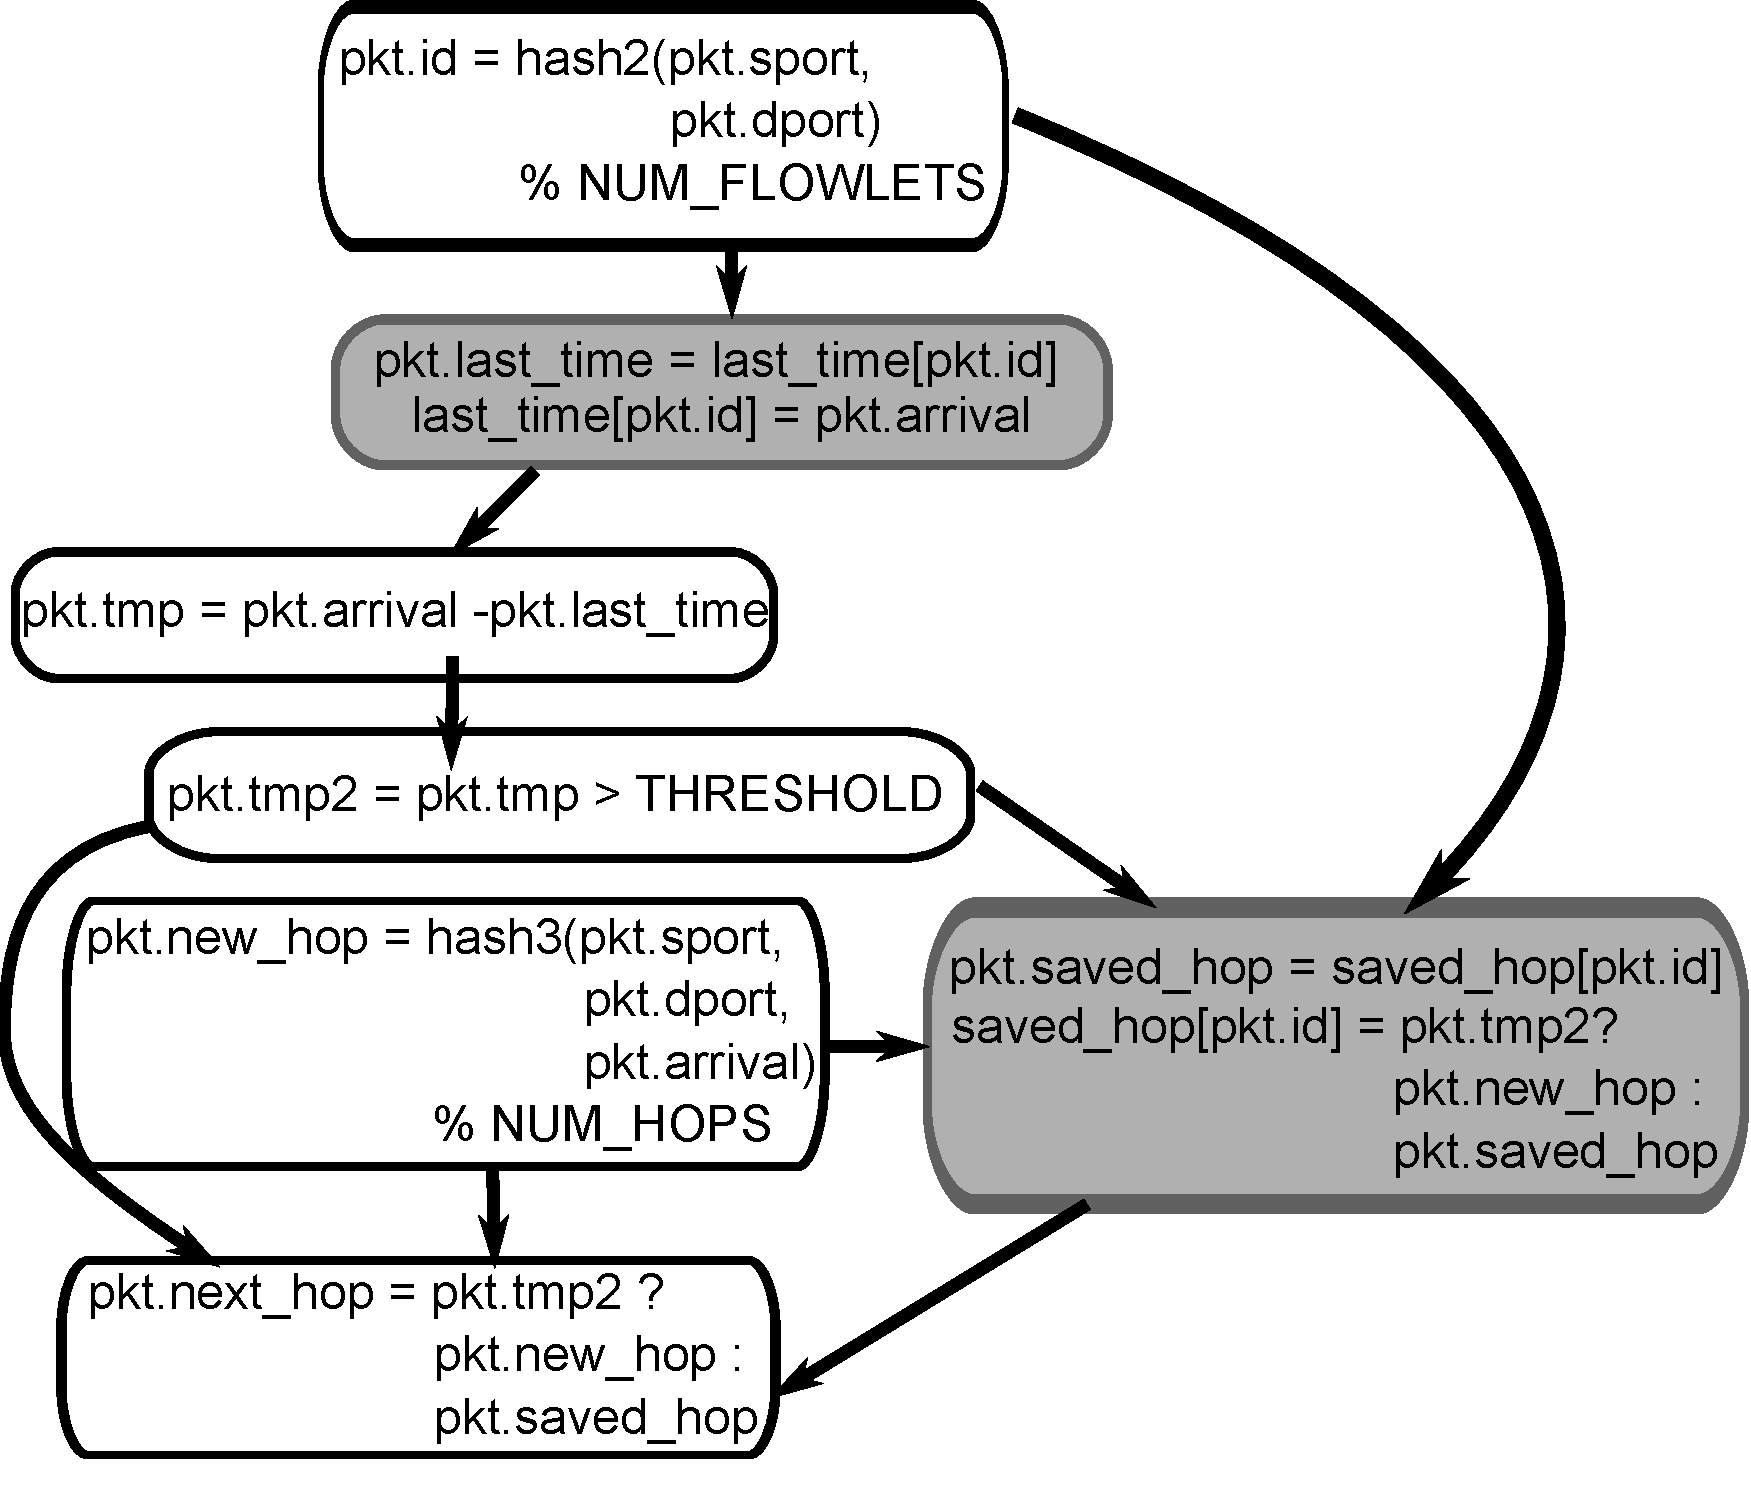
\includegraphics[width=0.8\columnwidth]{scc.pdf}
\caption{DAG after condensing SCCs.}
\label{fig:partitioning_after}
\end{subfigure}
\caption{Code Pipelining}
\label{fig:pipelining}
\end{figure*}

\subsection{Related compiler techniques}
\label{ss:related_compiler}
%%\ac{Why is this section here as opposed to the related work? Are we claiming novelty in
%%the rewriting techniques here? The differences seem incremental to me.}
%%Anirudh->Alvin: I think it's useful to have it here because we explicitly say that we reuse many compiler
%%techniques and its interesting to compare and contrast them specifically.
%%I don't have a religious opinion on this.

The \pktlanguage compiler employs many techniques from the compiler literature,
but adapts and simplifies them in new ways to suit the domain of line-rate
switches (Table~\ref{tab:prior_compiler}). The use of SCCs is inspired by
software pipelining for VLIW architectures~\cite{software_pipelining, rau}. The size
of the largest SCC affects the {\em maximum throughput} of the pipelined loop
in software pipelining. For \pktlanguage, it affects the {\em circuit area} of
the atom required to run a program at line rate. \pktlanguage trades off an
increase in space for line-rate performance.

Program synthesis was used for code generation in
Chlorophyll~\cite{chlorophyll}.  Code generation for \pktlanguage shares
similar goals as technology mapping~\cite{micheli, flowmap, spectransform} and
instruction selection~\cite{muchnik}.  However, prior work maps a code sequence
to \textit{multiple} instructions/tiles, using heuristics to minimize
instruction count. Domino's problem is simpler: we map each codelet to a single
atom using SKETCH.  The simpler problem allows a non-heuristic solution: if
there is any way to map the codelet to an atom, SKETCH will find it.

Branch removal resembles if-conversion~\cite{if_conversion}, a
technique used in vectorizing compilers. This procedure is easier in Domino
because there is no backward control transfer (goto, break,
continue). Domino's SSA computation operates on straight-line code and doesn't
 handle branches, which considerably complicate SSA algorithms~\cite{ssa}.

\begin{table}[!t]
  \begin{scriptsize}
    \begin{tabular}{|p{0.1\textwidth}|p{0.1\textwidth}|p{0.2\textwidth}|}
  \hline
  Technique & Prior Work & Differences \\
  \hline
  Conversion to straight-line code & If Conversion~\cite{if_conversion} & No backward control flow (gotos, break, continue) \\
  \hline
  SSA & Cytron et. al~\cite{ssa} & SSA runs on straight-line code with no branches \\
  \hline
  Strongly Connected Components & Lam~\cite{software_pipelining}, Rau and Glaeser~\cite{rau} & Scheduling in space vs. time \\
  \hline
  Code generation using program synthesis & Chlorophyll~\cite{chlorophyll}, technology mapping~\cite{micheli, flowmap, spectransform}, instruction selection~\cite{muchnik} & Optimal vs. best-effort mapping; One-to-one mapping vs. tiling \\
  \hline
  \end{tabular}
  \end{scriptsize}
  \caption{Domino's compiler in relation to prior work}
  \label{tab:prior_compiler}
\end{table}
